\section{Examples in Dummit}

$G$ is a finite group.

\subsection{Trivial representation}

Let $V$ be a 1-dimensional vector space over $F$ and make $V$ into an $FG$ -module by letting $gv=v$ for all $g\in G$ and $v\in V$. This module affords the representation
\[
\varphi :G\to \mathrm{GL}(V)
\]
to be trivial, i.e. taking $g$ to $1$ (the $1\times1$ identity matrix). The trivial representation has degree 1 and if $\lvert G \rvert>1$, it is \textbf{not faithful}.

\subsection{Regular representation}

Let $V=FG$ be a $FG$ -module, then $V$ affords a representation
\[
\varphi:G\to \mathrm{GL}(V)
\]
where $\varphi_{g}:g_i\mapsto g\cdot g_i$. $\varphi$ has degree equal to $\lvert G \rvert$, and it's always faithful. The matrix $R_{g}$ has a 1 in row $i$ and column $j$ if $gg_j=g_i$, and has 0's in all other positions.

\subsection{Permutation representation}

Let $G=S_n$, $V$ be an $n$ -dimensional vector space over $F$ with basis $e_1,e_2,\dots,e_n$. Let $S_n$ act on $V$ by defining for each $\sigma\in S_n$
\[
\sigma \cdot e_i=e_{\sigma(i)}\qquad 1\leq i\leq n
\]
This provides an \underline{injective} homomorphism of $S_n$ into $\mathrm{GL}(V)$. Hence $V$ is an $FS_n$ -module. $R_{\sigma}$ has a 1 in row $i$ and column $j$ if $\sigma(j)=i$.

\subsection{Composition to create new representation}

If $\psi :H\to \mathrm{GL}(V)$ is any representation of $H$ and $\varphi:G\to H$ is any group homomorphism, then the composition $\psi \circ \varphi$ is a representation of $G$.

\subsection{Degree 1 representation}

Any homomorphism of $G$ into the multiplication group $F^{\times}=\mathrm{GL}_{1}(F)$ is a degree 1 (matrix) representation.

For example, suppose $G= \left< g \right>\cong \mathbb{Z}_n$ is the cyclic group of order $n$ and $\zeta$ is a fixed $n^{\text{th}}$ root of 1 in $F$. Let $g^{i}\mapsto \zeta^{i}$, for all $i\in \mathbb{Z}$. This representation of $\left< g \right>$ is a faithful representation if and only if $\zeta$ is a primitive $n^{\text{th}}$ root of 1.

\subsection{Dihedral representation}

For $D_{2n}=\left< r,s\mid r^{n}=s^2=1,rsr=s \right>$, it has the faithful representation
\[
r\mapsto R_{r}=\begin{pmatrix}
\cos\frac{2\pi}{n} & -\sin\frac{2\pi}{n} \\
\sin\frac{2\pi}{n} & \cos\frac{2\pi}{n}
\end{pmatrix}\qquad s\mapsto R_{s}=\begin{pmatrix}
0 & 1 \\
1 & 0
\end{pmatrix}
\]
\subsection{Quaternion representation}

For $Q_8= \left< i,j\mid i^{4}=j^{4}=1,i^2=j^{2},jij=i \right>$, it has the faithful $\mathbb{C}$ -linear representation
\[
R_{i}=\begin{pmatrix}
\sqrt{ -1 } & 0 \\
0 & -\sqrt{ -1 }
\end{pmatrix}\qquad R_{j}=\begin{pmatrix}
0 & -1 \\
1 & 0
\end{pmatrix}
\]
And a 4-dimensional faithful $\mathbb{R}$ -linear representation is given by
\[
R_i=\begin{pmatrix}
0 & -1 & 0 & 0 \\
1 & 0 & 0 & 0 \\
0 & 0 & 0 & -1 \\
0 & 0 & 1 & 0
\end{pmatrix}\qquad R_j=\begin{pmatrix}
0 & 0 & -1 & 0 \\
0 & 0 & 0 & 1 \\
1 & 0 & 0 & 0 \\
0 & -1 & 0 & 0
\end{pmatrix}
\]
\begin{note}
Let $V=\mathbb{R}^{4}$, $F=\mathbb{R}$, $G=Q_8$.
\end{note}
\subsection{\texorpdfstring{$\mathbb{F}_{p}$}{mathbbF_p} -linear representation (modular representations)}

Suppose $H\lhd G$ and $H$ is an elementary abelian $p$ -group for some prime $p$. Let $V=H$ be a vector space over $\mathbb{F}_{p}$, where scalar $a\in \mathbb{F}_{p}$ acts on the group element $v\in V$ by $a\cdot v=v^{a}\in V$. The conjugation action of $g\in G$ on $V$ is $\mathbb{F}_{p}$ -linear because
\[
g\cdot(a\cdot v)=g\cdot(v^{a})=\mathrm{Ad}_{g}(v^{a})=gv^{a}g^{-1}=(gvg^{-1})^{a}=(\underbrace{ \mathrm{Ad}_{g}v }_{ \in H })^{a}\in V
\]
Then $V$ is an $\mathbb{F}_{p}G$ -module. The kernel of thsi representation is $C_{G}(H)\supset H$.

\section{Examples in Representations and Characters of Groups Gordon James}

See Representations and Characters of Groups Gordon James.

\subsection{Example 1}

Let $G=D_{12}=\left\langle a, b: a^6=b^2=1, b^{-1} a b=a^{-1}\right\rangle$. Define the matrices $A, B, C, D$ over $\mathbb{C}$ by
\[
\begin{gathered}
A=\left(\begin{array}{ll}
\mathrm{e}^{\mathrm{i} \pi / 3} & 0 \\
0 & \mathrm{e}^{-\mathrm{i} \pi / 3}
\end{array}\right), B=\left(\begin{array}{ll}
0 & 1 \\
1 & 0
\end{array}\right), \\
C=\left(\begin{array}{cl}
1 / 2 & \sqrt{ 3}  / 2 \\
-\sqrt{3 }  / 2 & 1 / 2
\end{array}\right), D=\left(\begin{array}{rr}
1 & 0 \\
0 & -1
\end{array}\right) .
\end{gathered}
\]
Prove that each of the functions $\rho_k: G \rightarrow \operatorname{GL}(2, \mathbb{C})(k=1,2,3,4)$, given by
\[
\begin{aligned}
& \rho_1: a^r b^s \rightarrow A^r B^s \\
& \rho_2: a^r b^s \rightarrow A^{3 r}(-B)^s \\
& \rho_3: a^r b^s \rightarrow(-A)^r B^s \\
& \rho_4: a^r b^s \rightarrow C^r D^s \quad(0 \leqslant r \leqslant 5,0 \leqslant s \leqslant 1)
\end{aligned}
\]
is a representation of $G$. Which of these representations are faithful? Which are equivalent?
\begin{proof}
It suffices to check that
\[
\rho(A)^{6}=\rho(b)^{2}=1,\qquad \rho(b)^{-1}\rho(a)\rho(b)=\rho(a)^{-1}
\]
which is routine. Since
\[
\ker \rho_1=\{ 1 \},\ker \rho_2=\{ 1,a^2,a^{4} \},\ker \rho_3=\{ 1 \},\ker \rho_4=\{ 1 \}
\]
$\rho_1,\rho_3,\rho_4$ are faithful.
\[
\rho_1\simeq \rho_3\simeq \rho_4
\]
Since their matrix representations have the same Jordan Canonical form.
\end{proof}

\subsection{Example 2}

Let $G$ be the dihedral group $D_8=\left\langle a, b: a^4=b^2=1, b^{-1} a b=\right.$ $\left.a^{-1}\right\rangle$. Define the matrices $A$ and $B$ by
\[
A=\left(\begin{array}{rr}
0 & 1 \\
-1 & 0
\end{array}\right), B=\left(\begin{array}{rr}
1 & 0 \\
0 & -1
\end{array}\right)
\]
And check that
\[
A^4=B^2=I, B^{-1} A B=A^{-1}
\]
It follows (see Example 1.4) that the function $\rho: G \rightarrow \mathrm{GL}(2, F)$ which is given by
\[
\rho: a^i b^j \rightarrow A^i B^j \quad(0 \leqslant i \leqslant 3,0 \leqslant j \leqslant 1)
\]
is a representation of $D_8$ over $F$. The degree of $\rho$ is $2$.

The matrices $g \rho$ for $g$ in $D_8$ are given in the following table:

\begin{table}[h]
	\centering
	\begin{tabular}{|c|c|c|c|c|}
		\hline
		$g$ & 1 & $a$ & $a^2$ & $a^3$ \\
		\hline
		$g \rho$ & $\left(\begin{array}{ll}1 & 0 \\ 0 & 1\end{array}\right)$ & $\left(\begin{array}{rr}0 & 1 \\ -1 & 0\end{array}\right)$ & $\left(\begin{array}{rr}-1 & 0 \\ 0 & -1\end{array}\right)$ & $\left(\begin{array}{rr}0 & -1 \\ 1 & 0\end{array}\right)$ \\
		\hline
		$g$ & $b$ & $a b$ & $a^2 b$ & $a^3 b$ \\
		\hline
		$g \rho$ & $\left(\begin{array}{rr}1 & 0 \\ 0 & -1\end{array}\right)$ & $\left(\begin{array}{rr}0 & -1 \\ -1 & 0\end{array}\right)$ & $\left(\begin{array}{rr}-1 & 0 \\ 0 & 1\end{array}\right)$ & $\left(\begin{array}{ll}0 & 1 \\ 1 & 0\end{array}\right)$ \\
		\hline
	\end{tabular}
\end{table}
Let
\[
T=\frac{1}{\sqrt{ 2 }}\begin{pmatrix}
1 & 1  \\
 i & -i 
\end{pmatrix} 
\]
Then
\[
T^{-1}AT=\begin{pmatrix}
i & 0 \\
0 & -i 
\end{pmatrix}\qquad T^{-1}BT=\begin{pmatrix}
0 & 1 \\
1 & 0
\end{pmatrix}
\]
So we obtain another representation $\sigma$ of $D_8$ for which
\[
a\sigma=\begin{pmatrix}
 i & 0 \\
0 & -i 
\end{pmatrix}\qquad b\sigma=\begin{pmatrix}
0 & 1  \\
1 & 0
\end{pmatrix}
\]
\subsection{Example 3}

Let $\rho$ be a representation of the group $G$. Suppose that $g$ and $h$ are elements of $G$ such that $(g \rho)(h \rho)=(h \rho)(g \rho)$. Does it follow that $g h=h g ?$
\[
(g \rho)(h \rho)=(h \rho)(g \rho)\iff (ghg^{-1}h^{-1})\rho=I\iff ghg^{-1}h^{-1}\in \ker \rho
\]
If $\rho$ is faithful then $gh=hg$. Otherwise, $g,h$ may not commute.

\subsection{Exercises}

\begin{exercise}[Yau-2024]
\begin{figure}[H]
\centering
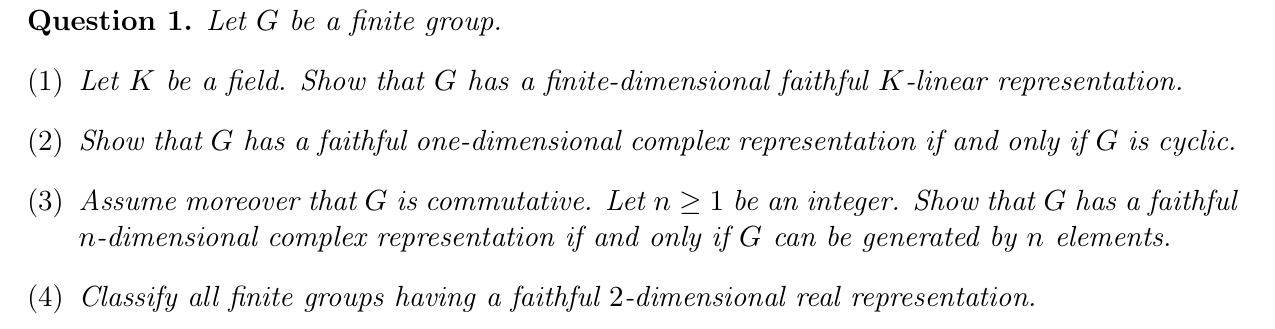
\includegraphics[width=\textwidth]{group-representation-2025050411.png}
% \caption{}
\label{}
\end{figure}
\end{exercise}
(1)
$\lvert G \rvert=n$, $G=\{ g_1,\dots,g_n \}$. Let $V$ be a $K$ -vector space whose basis is $\{ e_{g_1},\dots,e_{g_n} \}$. The dimension of $V$ is $\dim_{K}(V)=\lvert G \rvert$. More formally,
\[
V=\bigoplus_{g\in G}Ke_{g}
\]
$V$ is a finite vector space over $G$. Define the mapping (we will show that it's a representation),
\[
\rho:G\to \mathrm{Hom}(V,V)\qquad g\to \rho_{g}
\]
where $\rho_{g}: e_{h}\mapsto e_{gh}$. We can extend the action linearly to any $v=\sum_{h\in G}^{}\alpha_{h}e_{h}\in V$, by letting
\[
\rho_{g}(v)=\sum_{h\in G}\alpha_{h}e_{gh}
\]
To show that it's a homomorphism, we have
\[
\rho_{gg'}(e_{h})=e_{gg'h}=(\rho_{g}\circ \rho_{g'})(e_{h})\qquad \forall h\in G
\]
To show that the representation is faithful, consider the kernel
\[
\ker \rho=\{ g\in G:\rho(g)=id \}
\]
For $g\in \ker \rho$,
\[
e_{gh}=\rho_{g}(e_{h})=e_{h}\qquad \forall h\in G
\]
Then we have
\[
gh=h\qquad \forall h\in G\implies g=e
\]
Thus $\ker \rho=\{ e \}$. The representation is faithful.

(2)
If $G$ is cyclic with order $n$, and $G= \left< g \right>$, then the mapping
\[
\rho:G\to \mathrm{Hom}(\mathbb{C},\mathbb{C})\qquad g^{r}\mapsto e^{ 2\pi ir/n }
\]
is a faithful representation.

If $G$ has a faithful one-dimensional complex representation,
\[
\rho:G\to \mathrm{Hom}(\mathbb{C},\mathbb{C})\qquad g\mapsto \rho_{g}
\]
$\lvert G \rvert=n$, then $\rho (g)^{n}=1,\forall g\in G$. Thus every $\rho_{g}$ lies in the set of $n^{\text{th}}$ roots of unity, which has size $n$. Since $\rho$ is faithful, $\rho_{g}\neq \rho_{h}$ for $g\neq h$. Then $\rho(G)=\{ \mu _n \}$ is cyclic. Hence $G$ is cyclic.

(3)
If $G$ can be generated by $g_1,\dots,g_n$, then for any $g\in G$, we have
\[
g=g_1^{r_1}\dots g_n^{r_n}
\]
Assume that $g_i^{\alpha _i}=e$ for every $i$, then the mapping
\[
\rho:G\to \mathrm{Hom}(\mathbb{C}^{n},\mathbb{C}^{n})\qquad g\mapsto \mathrm{diag}\{ e^{ 2\pi ir_1/\alpha_1 },\dots e^{ 2\pi i r_n/\alpha _n } \}
\]
is a faithful $n$ -dimensional complex representation.

If $G$ has a faithful $n$ -dimensional complex representation,
\[
\rho:G\to \mathrm{Hom}(\mathbb{C}^{n},\mathbb{C}^{n})\qquad g\mapsto \rho_{g}
\]
$\rho_{g}$ can be a diagonized matrix.
....

(4)
具有忠实的二维实表示的有限群的分类如下:

\begin{enumerate}
	\item 循环群 $C_n$( n 阶循环群),对于任意 $n \geq 1$ 。
	\item 二面体群 $D_m$( 2 m 阶二面体群,即正 m 边形的对称群),对于任意 $m \geq 1$ 。
\end{enumerate}

\begin{remark}
Let $(\rho, V)$ be a finite dimensional $\mathbb{C}$-representation of a finite group $G$. Consider the $G$-invariant subspace
\[
V^G:=\{v \in V \mid \rho(g)(v)=v \text { for all } g \in G\}
\]	\begin{enumerate}
		\item Show that $\operatorname{dim} V^G$ is the same as the multiplicity of the trivial representation appearing in $V$.
		\item Show that $\operatorname{dim} V^G=\frac{1}{|G|} \sum_{g \in G} \chi_\rho(g)$.
		\item Construct a surjective map $\phi: V \rightarrow V^G$, expressed in terms of a linear combination of linear operators $\rho(g)$ for $g \in G$, such that $\phi^2=\phi$ (i.e. $\phi$ is a projection) and $\phi$ is a homomorphism.
	\end{enumerate}
\end{remark}
\begin{figure}[H]
\centering
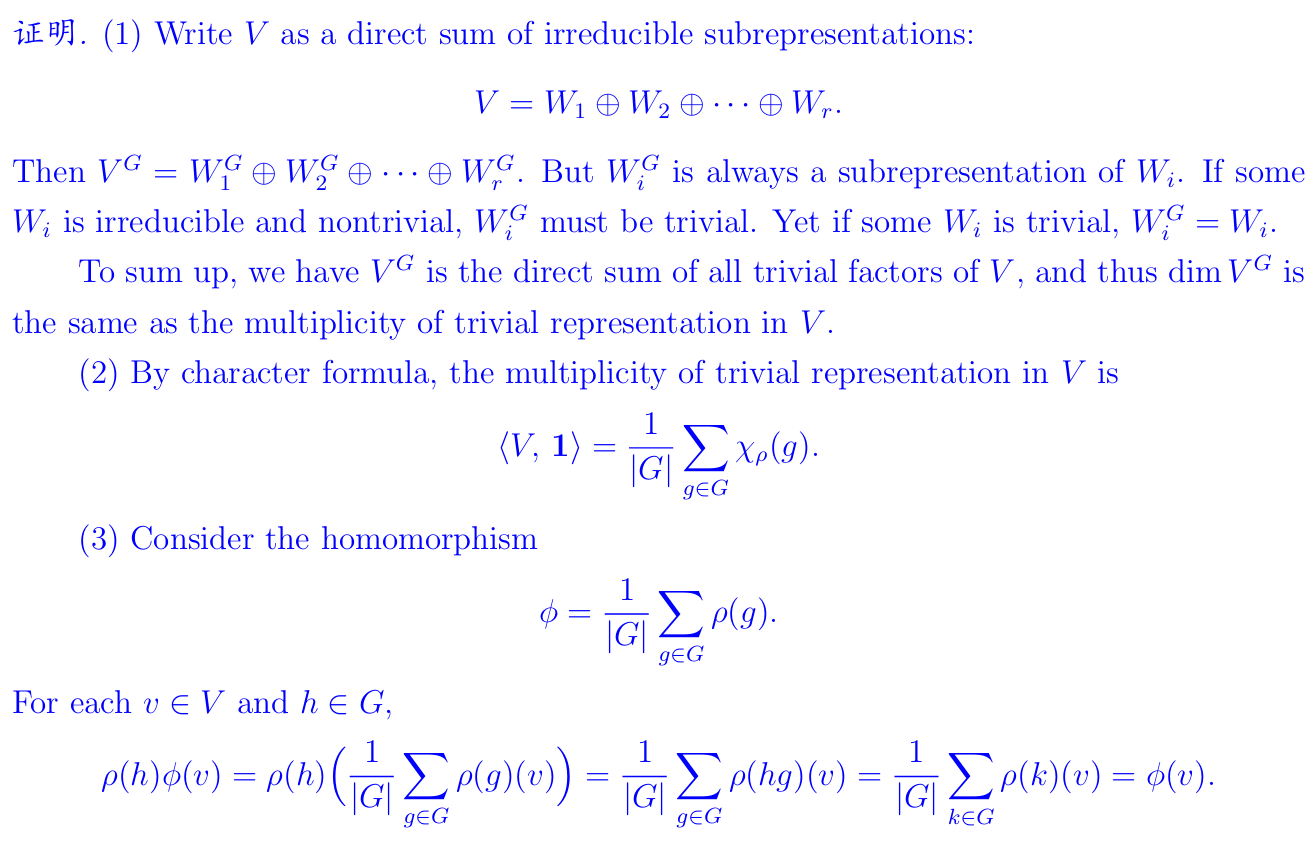
\includegraphics[width=\textwidth]{group-representation-2025051012.png}
% \caption{}
\label{}
\end{figure}
\begin{figure}[H]
\centering
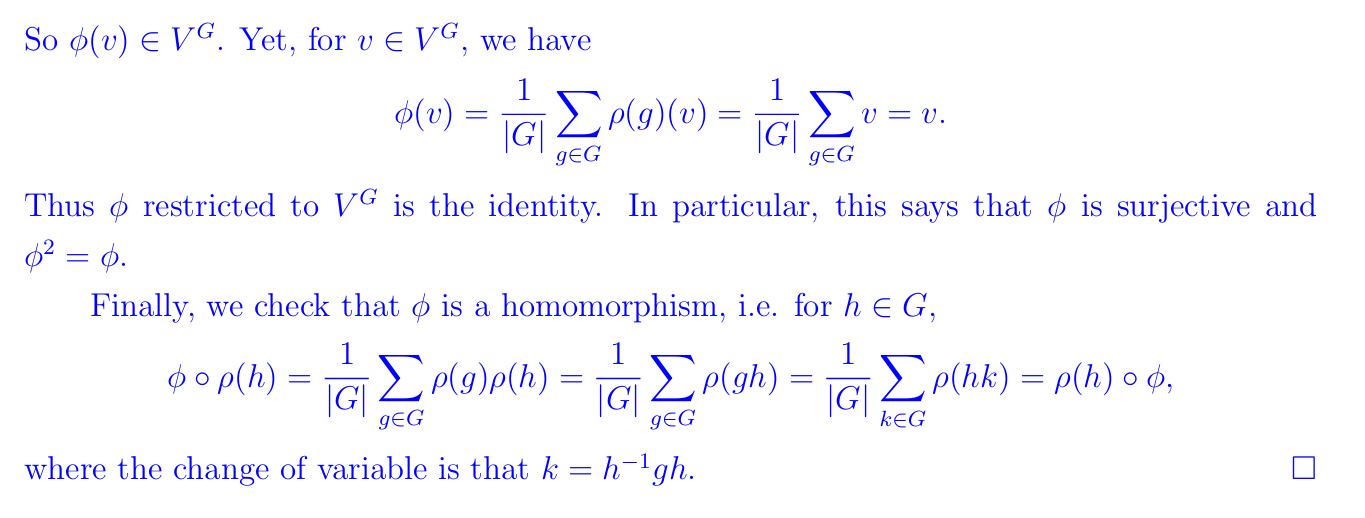
\includegraphics[width=\textwidth]{1-group-representation-2025051012.png}
% \caption{}
\label{}
\end{figure}
